\documentclass[]{article}
\usepackage{geometry}
\geometry{margin=1in}
%opening
\usepackage{booktabs}
\usepackage[scale=2]{ccicons}

\usepackage{graphicx}
\usepackage{subcaption}
\graphicspath{Photos/}
\usepackage{amsmath,amsfonts,amssymb}
\usepackage{listings}
\usepackage{xcolor}   % for \textcolor
\usepackage{hyperref}
\usepackage{placeins}
%opening
\title{Failure Analysis of a 1/4" Ball Valve}
\author{Ghulam Haider, Daniel Moses}

\begin{document}

\maketitle

\begin{abstract}
	
	Premature ball valve failure can lead to many undesirable outcomes including system downtime, quality issues, and safety hazards. This project investigates the failure modes of a severely eroded 1/4" ball valve. A thorough investigation of failure progression for this particular valve and its components is carried out to determine the failure chain and root cause. Finally, based on this investigation, recommendations for design improvements and best practices for application are made.
	

\end{abstract}
\tableofcontents
\pagebreak
\section{Summary of Conclusions and Recommendations}
A decommissioned 1/4" ball valve from the University of Tulsa’s north campus showed signs of extreme erosion and corrosion damage.The valve likely failed to seal for an unknown length of time and was eventually replaced due to leakage from the valve body. The primary failure mechanisms include both operational errors and fluid characteristics.

\textbf{Summary of Failure Causes:}
\begin{itemize}
	\item The valve was left partially open for prolonged throttling applications. This resulted in extensive fluid and cavitation erosion. 
	\item Abrasive particles (sand) were embedded in the seal surfaces. These particles scratched grooves into the ball and prevented proper sealing.
	\item Corrosive solvents weakened brass components through a de-alloying corrosion process. Corrosion was further expedited by cavitation.
\end{itemize}

Ball valves are not intended for continuous throttling operations in this environment. Alternative valve selection is recommended if future leaks and frequent valve replacement are to be avoided.

\section{Introduction}
The ball valve for this study came from the University of Tulsa's north campus. The valve application, operating conditions, and length of service life were not known at the beginning of this study. The valve type and size suggest that the valve was most likely in service on an experimental erosion/corrosion (E/CRC) flow loop. These loops typically contain water with a mixture of other abrasive and/or corrosive additives. The particular application(s) for this valve included sand and salt additives, as discussed in Section 4. The goal of this analysis is to assess the viability of this valve for continued use in E/CRC applications. 


\subsection{Ball Valve Components and Operation}
Ball valves are used to control fluid flow in a line or pipe. Ball valves are different from many other types of valves, in that the valve does not impede flow when in the open position. While ball valves of varying design and complexity exist, this study will focus on floating ball valves similar to one found on north campus. 

A section view of a typical ball valve is shown in Figure \ref{fig:cutview}. As a fluid enters the valve from the left, it encounters a ball with a bored out hole. If the hole is in line with the pipe, the flow continues unimpeded (0\verb|%| pressure drop). If the hole is perpendicular to the pipe, the flow is stopped (100\verb|%| pressure drop). During opening and closing, the valve must pass through a state of being partially opened. As the flow enters a partially opened valve, the reduction in area induces a throttling effect. Ball valves are typically designed and used in on-off applications where the erosion effects due to partially opened flow states can be neglected.


\begin{figure}[h]
	\centering
	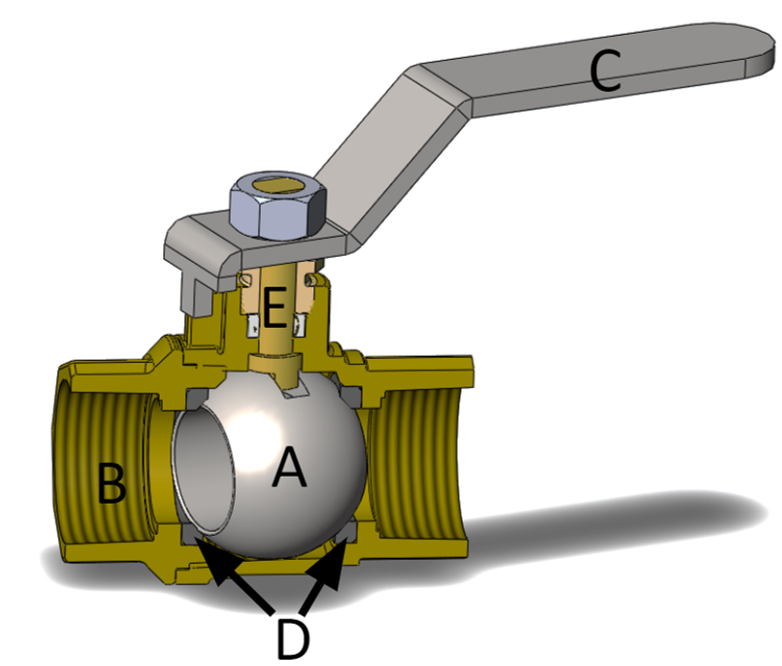
\includegraphics[width=0.33\linewidth]{Photos/CutView}
	\caption{Ball Valve Internal Mechanism. A: Ball; B: Valve Body; C: Handle; D: Seals; E: Stem}
	\label{fig:cutview}
\end{figure}

\section{Initial Visual Inspection}
Initial visual examination revealed several obvious areas of erosion within the valve. Some of the most severe damages are highlighted in Figure \ref{fig:Ball_Valve_as_Recieved}. 

\begin{figure}[htbp]
	\centering
	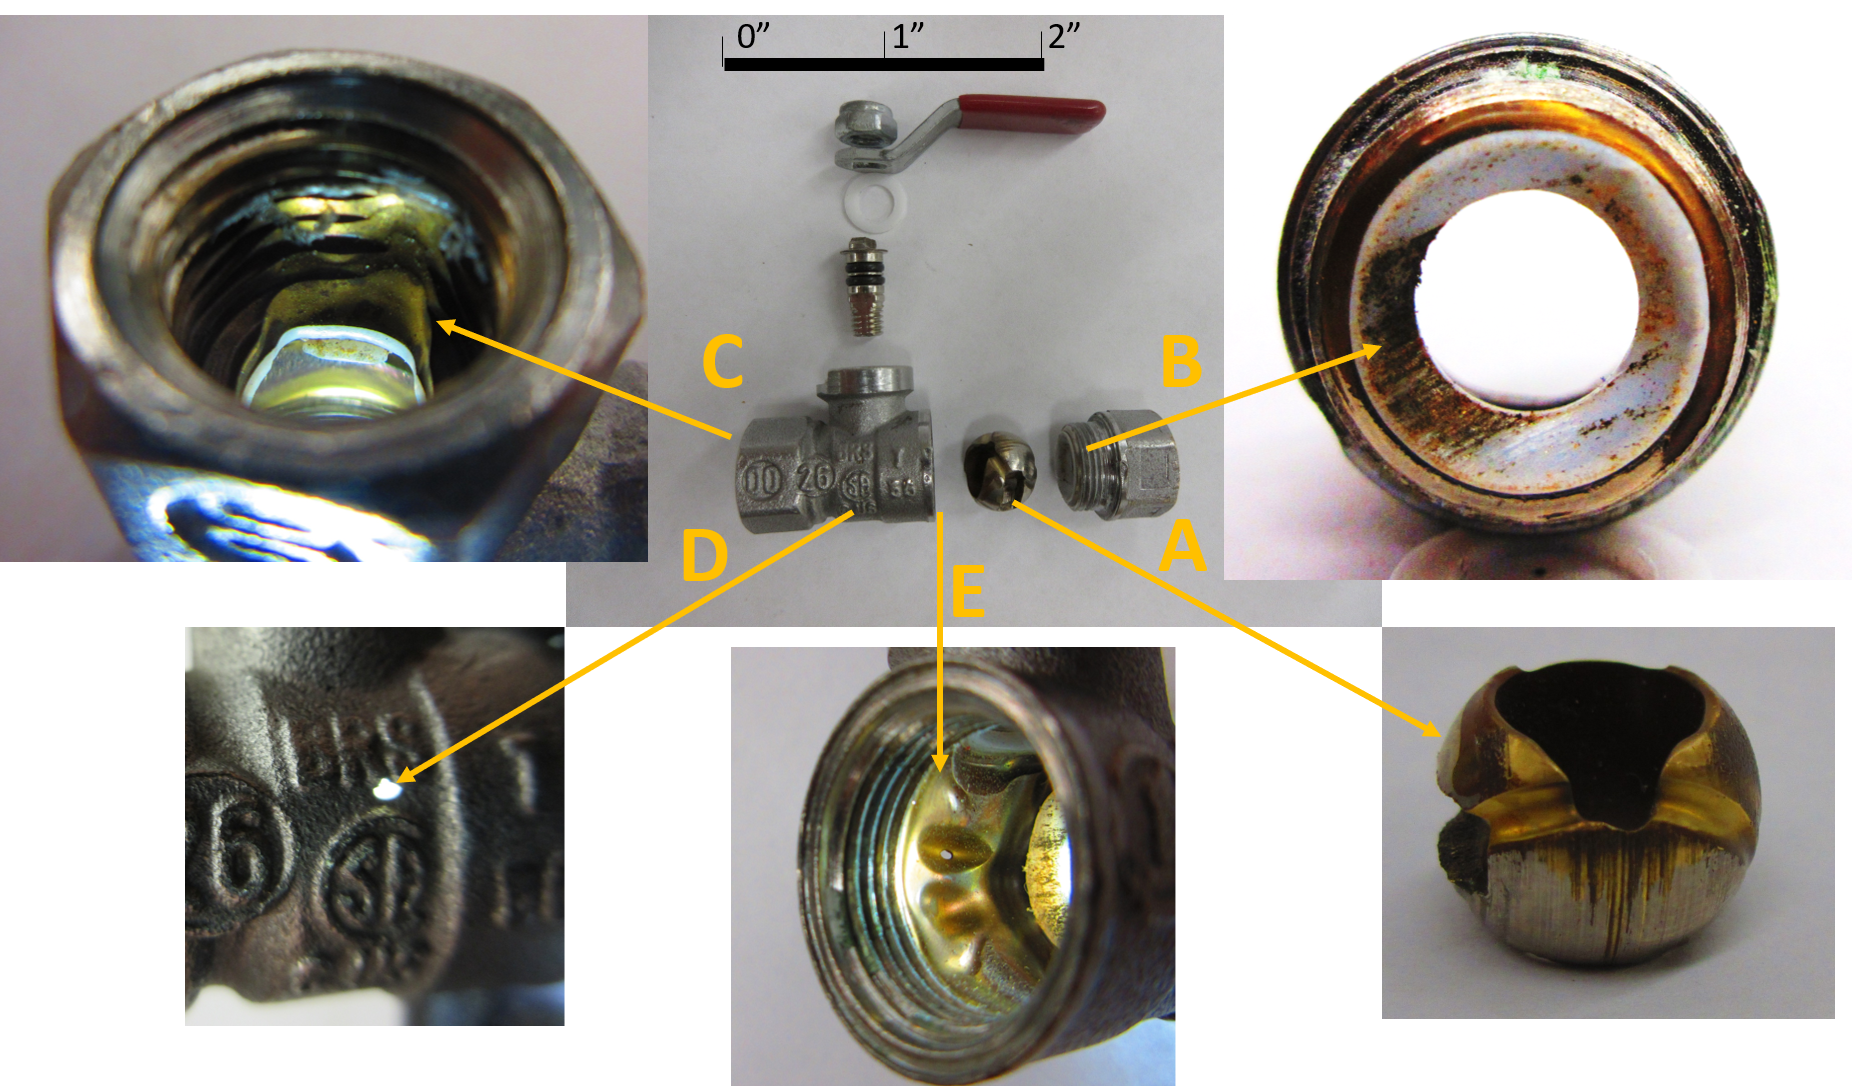
\includegraphics[width=0.95\linewidth]{Photos/Exploded_Callouts}
	\caption{A: Nickel plated brass ball; B: Nickel plated 1/4" brass nipple with Teflon seal; C: Erosion of valve body outlet; D: Pin hole outside valve body; E: Erosion of valve body inlet}
	\label{fig:Ball_Valve_as_Recieved}
\end{figure}
\subsection{Valve Ball}
The valve ball is a brass alloy 60-40 percent copper-zinc, respectively. The ball is externally coated with a thin nickel plating. Examination of the ball revealed several distinct erosion and corrosion patterns. Internal erosion was dominated by a single channel as shown in Figure \ref{fig:internalballerossion}. This channel was smooth and shiny in appearance. 
\begin{figure}[h]
	\centering
	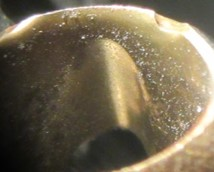
\includegraphics[width=0.4\linewidth]{Photos/internal_ball_erossion}
	\caption{Internal Ball Erosion}
	\label{fig:internalballerossion}
\end{figure}

Externally, the ball had 4 distinct areas of interest:
\begin{enumerate}
	\item Sealing faces
	\item Upstream edge
	\item Internal edge (1)
	\item Internal edge (2)
	\end{enumerate} 
The sealing faces consisted of the two opposite ball faces that contact the ball seals during opening and closing. These faces were characterized by several horizontal, parallel grooves. The grooves tended to have distinct shiny and dark lines distributed throughout. The upstream edge is the portion of the ball valve facing upstream when the valve is in the partially opened position. This face had a flattened appearance where the nickel plating had been worn away. The two internal edges are always between the valve seals as shown due to the 90 degree limitation of the ball rotation. Edge 1 had two symmetric groves running diagonally across the ball's outer face. The grooves were shiny in appearance and were both very smooth. Edge 2 was characterized by a rough, pock marked surface that was very dark in color. See Figure \ref{fig:ball} 

\begin{figure}[h]
	\centering
	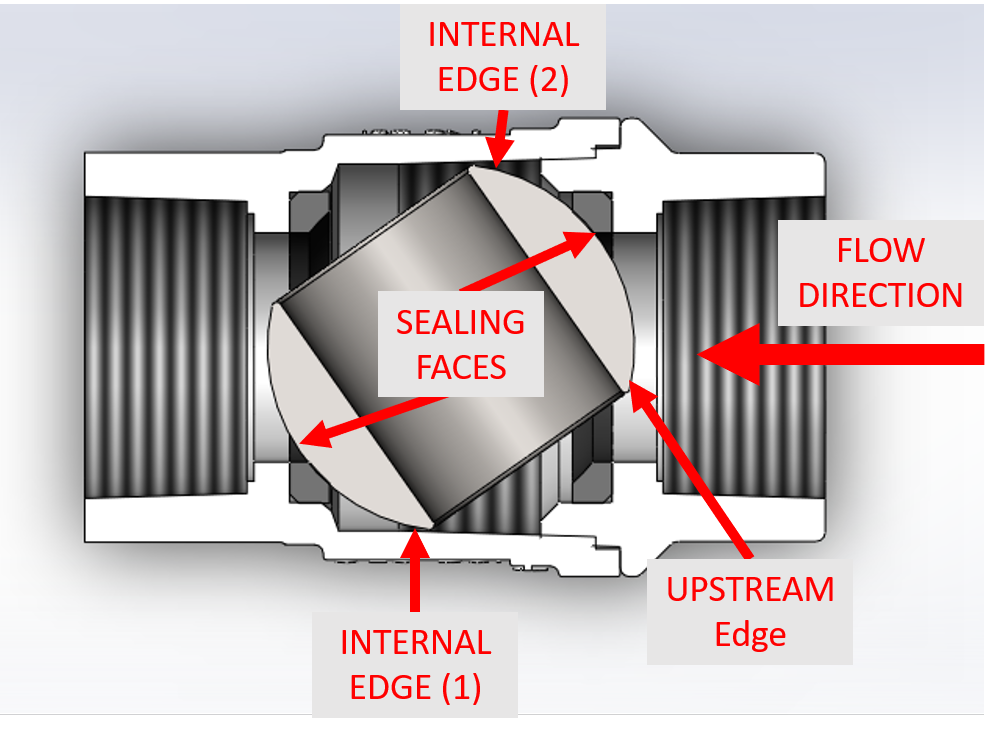
\includegraphics[width=0.7\linewidth]{Photos/Ball_Face_Callouts}
	\caption{Top View Valve Cross Section: External Ball Faces}
	\label{fig:ballfacecallouts}
\end{figure}

\begin{figure}
	\centering
	\begin{subfigure}[h]{0.4\textwidth}
		\includegraphics[width=\textwidth]{Photos/ball_seal_faces}
		\caption{Sealing Faces}
		\label{fig:sealingFaces}
	\end{subfigure}
	~ %add desired spacing between images, e. g. ~, \quad, \qquad, \hfill etc. 
	%(or a blank line to force the subfigure onto a new line)
	\begin{subfigure}[h]{0.4\textwidth}
		\includegraphics[width=\textwidth]{Photos/ball_upstream_face}
		\caption{Upstream Edge}
		\label{fig:upstream edge}
	\end{subfigure}
	~ %add desired spacing between images, e. g. ~, \quad, \qquad, \hfill etc. 
	%(or a blank line to force the subfigure onto a new line)
	
	\begin{subfigure}[h]{0.4\textwidth}
		\includegraphics[width=\textwidth]{Photos/ball_internal_edge_1}
		\caption{Internal Edge 1}
		\label{fig:Internal edge 1}
	\end{subfigure}
	~
	\begin{subfigure}[h]{0.4\textwidth}
	\includegraphics[width=\textwidth]{Photos/ball_internal_edge_2}
		\caption{Internal Edge 2}
		\label{fig:Internal edge 2}
	\end{subfigure}
	\caption{External Ball Features}\label{fig:ball}
\end{figure}

\subsection{Valve Seals}
The inlet and outlet seals were both characterized by 3 distinct regions. The 3 regions of the inlet seal in Figure \ref{fig:inletseal} are:
\begin{enumerate}
	\item Water inflow region (left)
	\item Continuous contact region (top and bottom)
	\item Mixed contact region (right)
\end{enumerate}
The water inflow region is the portion of the upstream seal fully exposed to fluid during opening and closing. The seal surface in this region is generally intact but is characterized by a layer of grainy residue. The continuous contact region is the portion of the seal that is always in contact with the ball. This region is smooth and shows little sign of damage or debris. The mixed contact region is also in continuous contact with the ball, but it differs from the continuous contact region in that the portion of the ball in contact with this region is intermittently exposed to the fluid. This region is characterized by numerous, scattered indentations in the seal. Some residue is present within the indents.

\begin{figure}
	\centering
	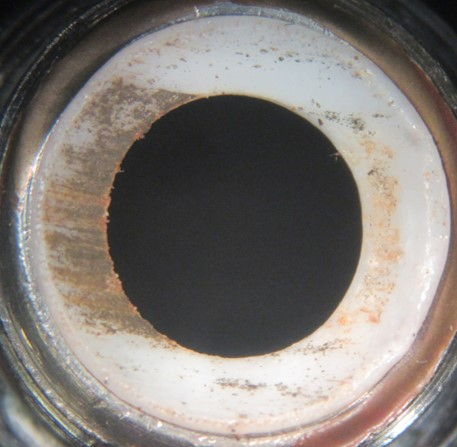
\includegraphics[width=0.4\linewidth]{Photos/Inlet_Seal}
	\caption{Valve Seal (Inlet)}
	\label{fig:inletseal}
\end{figure}

The outlet seal regions are shown in figure \ref{fig:outletseal} and include:
\begin{enumerate}
	\item Water outlet region (right)
	\item Continuous contact region (top and bottom)
	\item Back-flow region (left)
\end{enumerate}
The water outlet region is the portion of the downstream seal fully exposed to fluid during valve opening and closing. The distinguishing feature of this region is a portion of the seal protruding perpendicular to the surface. The continuous contact region is similar to the inlet seal. The back-flow region is the portion of seal that is in continuous contact with the ball. The seal's surface in this region is generally intact but is covered with a layer of grainy debris. 

\begin{figure}[h]
	\centering
	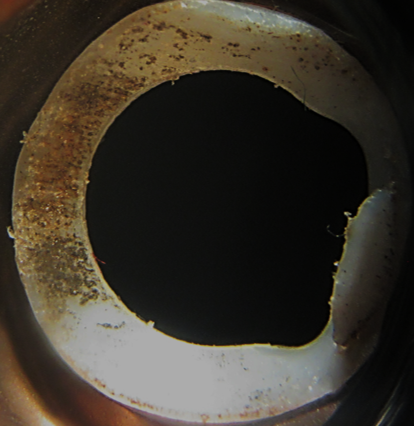
\includegraphics[width=0.4\linewidth]{Photos/Outlet_seal}
	\caption{Valve Seal (Outlet)}
	\label{fig:outletseal}
\end{figure}


\subsection{Valve Body}
The valve body has several distinct areas of damage. The inlet opening is shown in Figure \ref{fig:inlet}. The part of the wall exposed to upstream flow during valve opening and closing corresponds to the ball's internal edge 1 in Figure \ref{fig:ballfacecallouts}. The bowl-shaped indentations seen are smooth and shiny in appearance. The uppermost indentation has a small hole (1/32") where the wall material has been completely worn through. Additional material is eroded downstream of the indentations where seal undercutting is observed. 

The part of the valve exposed to downstream flow during valve opening and closing corresponds to the ball's internal edge 2  in Figure \ref{fig:ballfacecallouts}. Several smooth, shiny channels are present, and a dark, rough band extends from the bottom to the top of the valve. The valve outlet (Figure \ref{fig:bodyoutlet}) has a concentrated area of erosion on one side that is smooth and shiny in appearance.

\begin{figure}[h]
	\centering
	\begin{subfigure}[h]{0.4\textwidth}
		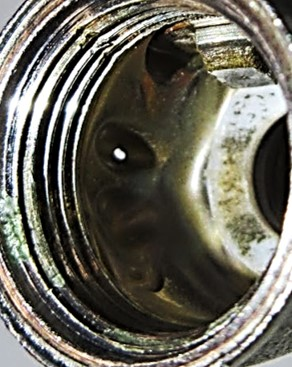
\includegraphics[width=\textwidth]{Photos/Body_sides}
		\caption{Upstream Exposure}
		\label{fig:bodysides}
	\end{subfigure}
	~
	\begin{subfigure}[h]{0.4\textwidth}
		\centering
		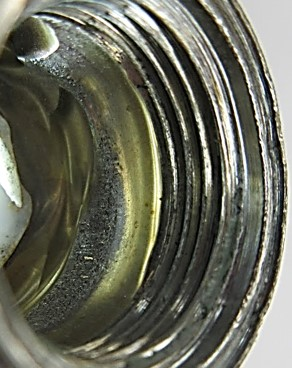
\includegraphics[width=\textwidth]{Photos/Body_side2}
		\caption{Downstream Exposure}
		\label{fig:bodyside2}
	\end{subfigure}

	\caption{Valve Inlet}\label{fig:inlet}
\end{figure}



\begin{figure}[h]
	\centering
	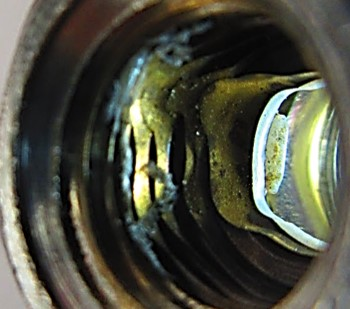
\includegraphics[width=0.6\linewidth]{Photos/Body_outlet}
	\caption{Valve Outlet}
	\label{fig:bodyoutlet}
\end{figure}
%(Laboratory Examinations)
\FloatBarrier
\subsection{SEM}
The valve ball and seal were examined under SEM with energy dispersion spectroscopy (EDS). Two images of the ball surface are shown in Figure \ref{fig:BallSEM}. Images (a) and (b) came from a darkened, rough portion of the ball surface as seen in Figure \ref{fig:ball}(d). EDS indicated predominately copper, carbon, and oxygen composition in the darkened, leftmost region of Figure \ref{fig:BallSEM}(a) and nickel in the lighter region to the right. The rough surface in (b) was not analyzed with EDS, but is believed to be primarily copper, carbon, and oxygen. EDS of Figure \ref{fig:BallSEM}(c) reported copper and zinc at an element ratio of 65\verb|%| to 35\verb|%| respectively. EDS also indicated small amounts of sodium and chlorine on the ball surface. EDS of the seal surface showed larger concentrations of sodium, chloride, and silicon, dispersed over the water inflow region of the seal in figure \ref{fig:inletseal}.

\begin{figure}[h]
	\centering
	\begin{subfigure}[h]{0.32\textwidth}
		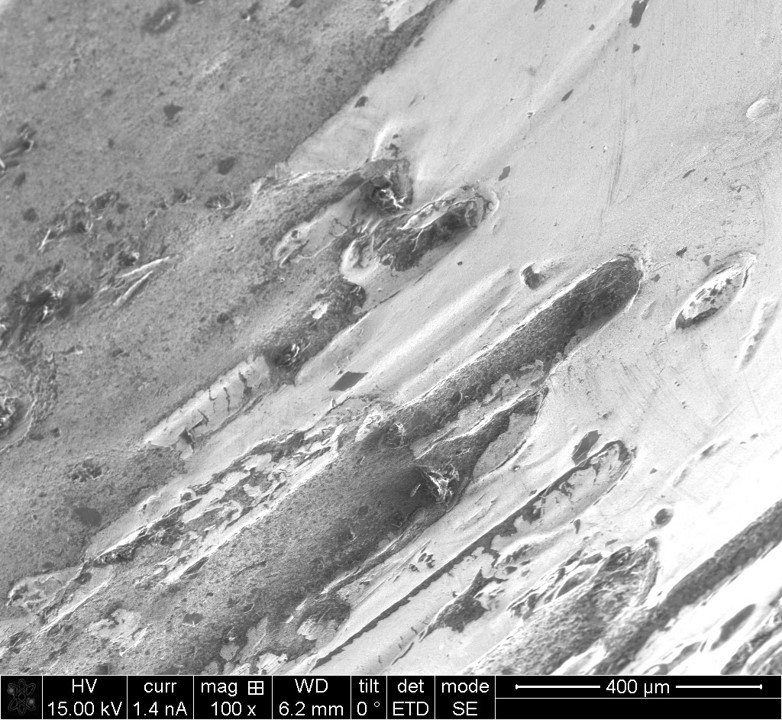
\includegraphics[width=\textwidth]{Photos/SEM_01}
		\caption{Gray-Cu,C,O; White-Ni}
		%\label{fig:SEMball1}
	\end{subfigure}
	~
	\begin{subfigure}[h]{0.32\textwidth}
		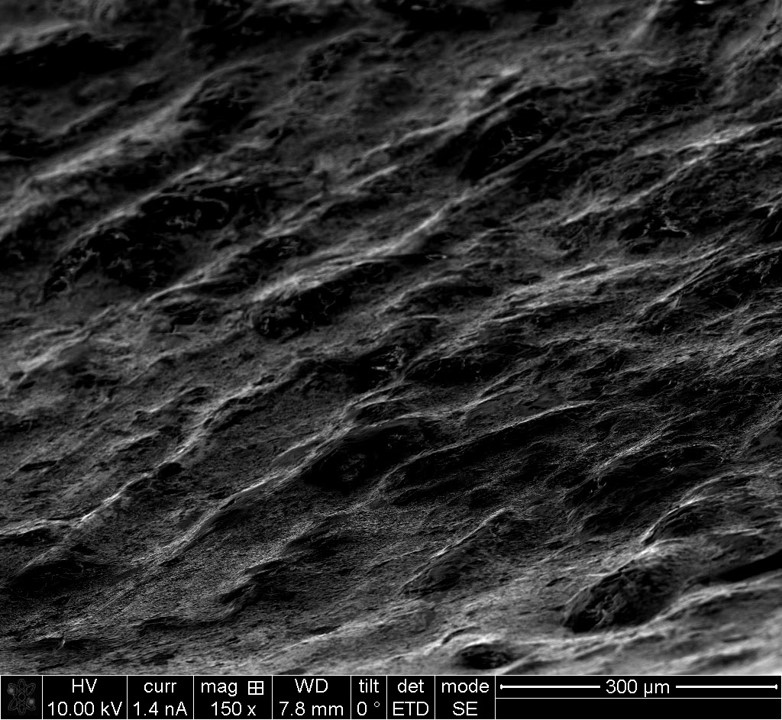
\includegraphics[width=\textwidth]{Photos/SEM_rough}
		\caption{Rough Surface}
		%\label{fig:SEMball2}
	\end{subfigure}
	\begin{subfigure}[h]{0.32\textwidth}
		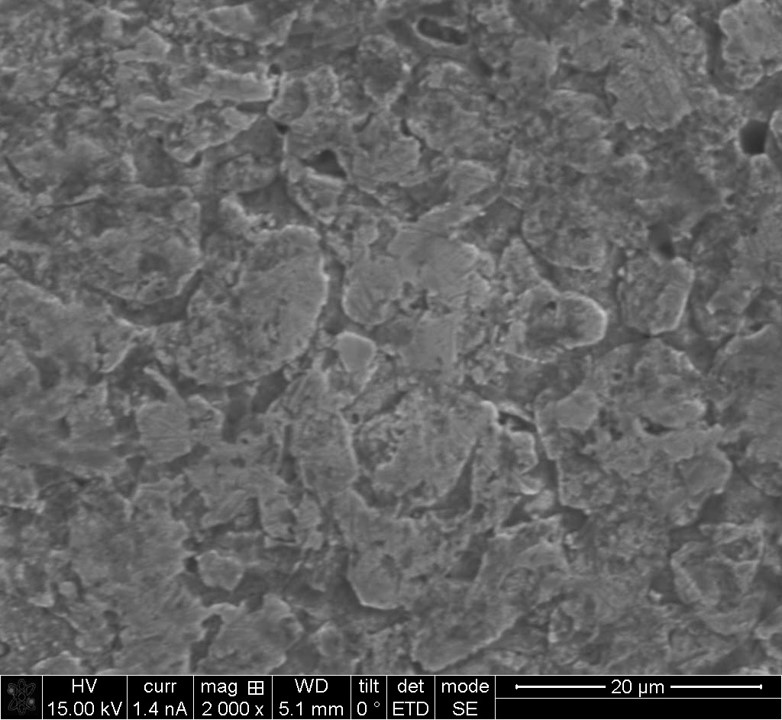
\includegraphics[width=\textwidth]{Photos/SEM_03}
		\caption{65-35 Zn-Cu}
		%\label{fig:SEMball2}
	\end{subfigure}
	\caption{Ball SEM Images}\label{fig:BallSEM}
\end{figure}

\section{Analysis:CFD}
A CFD study of the ball valve under investigation is conducted. While the actual operating conditions of this valve are unknown, it is assumed that this valve was operated on a water line with extensive throttling. CFD simulations using ANSYS/FLUENT 18.2 are performed in half-open position to simulate the effect of throttling on the mass flow rate through the valve as well as the pressure and velocity. Moreover, three different inlet velocities i.e. 15m/s, 25 m/s and 35 m/s are simulated as the actual velocity inlet information is unknown.
The continuity, momentum and turbulence generation, and destruction equations are solved by means of the Finite Volume commercial code FLUENT, assuming the hypotheses of steady–state, incompressible and isothermal flow. Flow solution is obtained through RNG k-ε model with enhanced wall treatment. Turbulent variables have been set by specifying the hydraulic diameter of the inlet port and a typical value of the turbulent intensity of \verb|5%|.The fluid is water with the following properties: density 998.2 kg/m3 and viscosity 0.001003 kg/m-s.

\subsection{Geometry and Computational Domain}
Figure \ref{fig:geometry} shows the schematic diagram of the ball valve which is used for this simulation.  The diameter of the valve is approximately 0.31 inch. 
\begin{figure}[h]
	\centering
	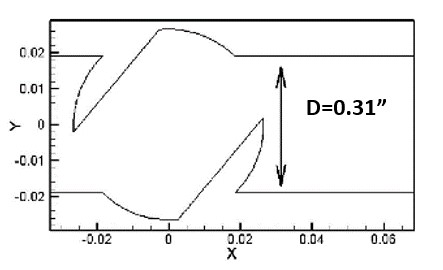
\includegraphics[width=0.7\linewidth]{Photos/Geometry}
	\caption{Schematic Diagram of Geometry}
	\label{fig:geometry}
\end{figure}

Figure \ref{fig:entiregeometry} shows the complete geometry of this cfd study. The entrance length from the upstream boundary to the valve is 20D. The downstream length from the valve to the outlet boundary is 10D.
\begin{figure}
	\centering
	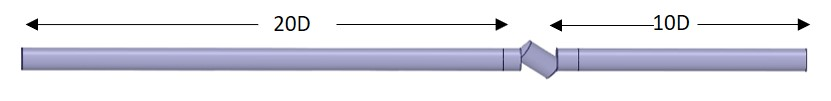
\includegraphics[width=0.7\linewidth]{Photos/Entire_Geometry}
	\caption{Complete Geometry}
	\label{fig:entiregeometry}
\end{figure}
Figure \ref{fig:Mesh} (a and b) shows the 3D computational domain utilized in numerical simulations. Flow domain was separated in three parts: Inlet portion, Ball-Valve, Outlet portion. This scheme was used to implement a hybrid mesh. Hex mesh was used on both inlet and outlet portions. Hexahedral elements are usually more efficient which results in faster solution time with better accuracy. Ball valve was meshed with tetrahedral elements as these type of elements are more suitable for complex geometries. In flow regions near the wall, inflated meshes are created. 
A uniform inlet velocity profile was specified at the entrance to the pipe. Length of the pipe was selected to be long enough for the fluid to be fully developed. On the downstream outflow face, a zero gradient pressure outlet was applied. On the wall, the boundary conditions are velocity impermeability and no slip, and the normal gradient of the pressure is assumed to be zero. Wall functions based on the law of the wall are used as boundary conditions for the turbulence modeling. The turbulence intensity at the entrance to the channel was set to be \verb|10%|. Heat transfer is not considered in these simulations.

\begin{figure}
	\centering
	\begin{subfigure}[h]{0.8\textwidth}
		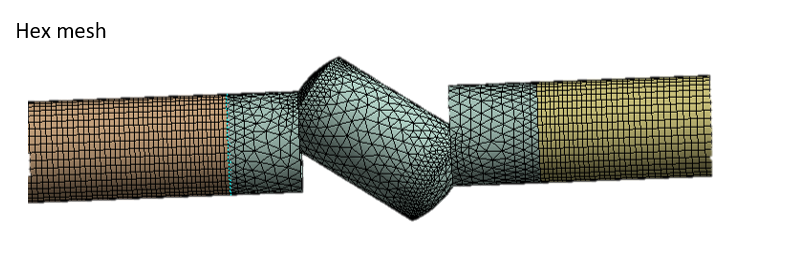
\includegraphics[width=\textwidth]{Photos/Flow_Domain}
		\caption{Meshing Scheme}
	\end{subfigure}
	~ %add desired spacing between images, e. g. ~, \quad, \qquad, \hfill etc. 
	%(or a blank line to force the subfigure onto a new line)
	
	\begin{subfigure}[h]{0.8\textwidth}
		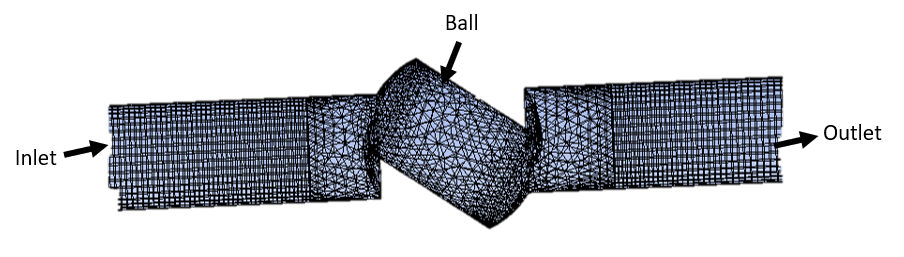
\includegraphics[width=\textwidth]{Photos/Wire_Frame}
		\caption{Wire Frame View}
	\end{subfigure}
	\caption{Flow Domain}\label{fig:Mesh}
\end{figure}
\FloatBarrier
\subsection{Results}
Figure \ref{fig:velocity} illustrates the velocity contours and path line flow pattern on a middle plane for different inlet velocities for the half-open position. For reference, velocity contours for a fully-open valve are also plotted. It can be observed that as the valve opening decreases, the vortex region increases. These plots also shows the recirculation behind the ball valve. This recirculation region contributes to the pressure drop across the valve as energy is dissipated in this region. Pressure drop increases with the increase in recirculation length. This recirculation length is affected by the valve position. This length increases as the valve opening is decreased. Systems with higher pressure drop expend more energy to maintain the same volumetric flow rate.

Similarly, figure \ref{fig:pressure} shows the static pressure distribution in the center plane. For reference, contours for a fully-open valve are also plotted. High pressure drop (Area of the reduced pressure and its extent) can be observed across the valve resulting in extremely low pressure regions within the flow domain. 
\begin{figure}
	\centering
	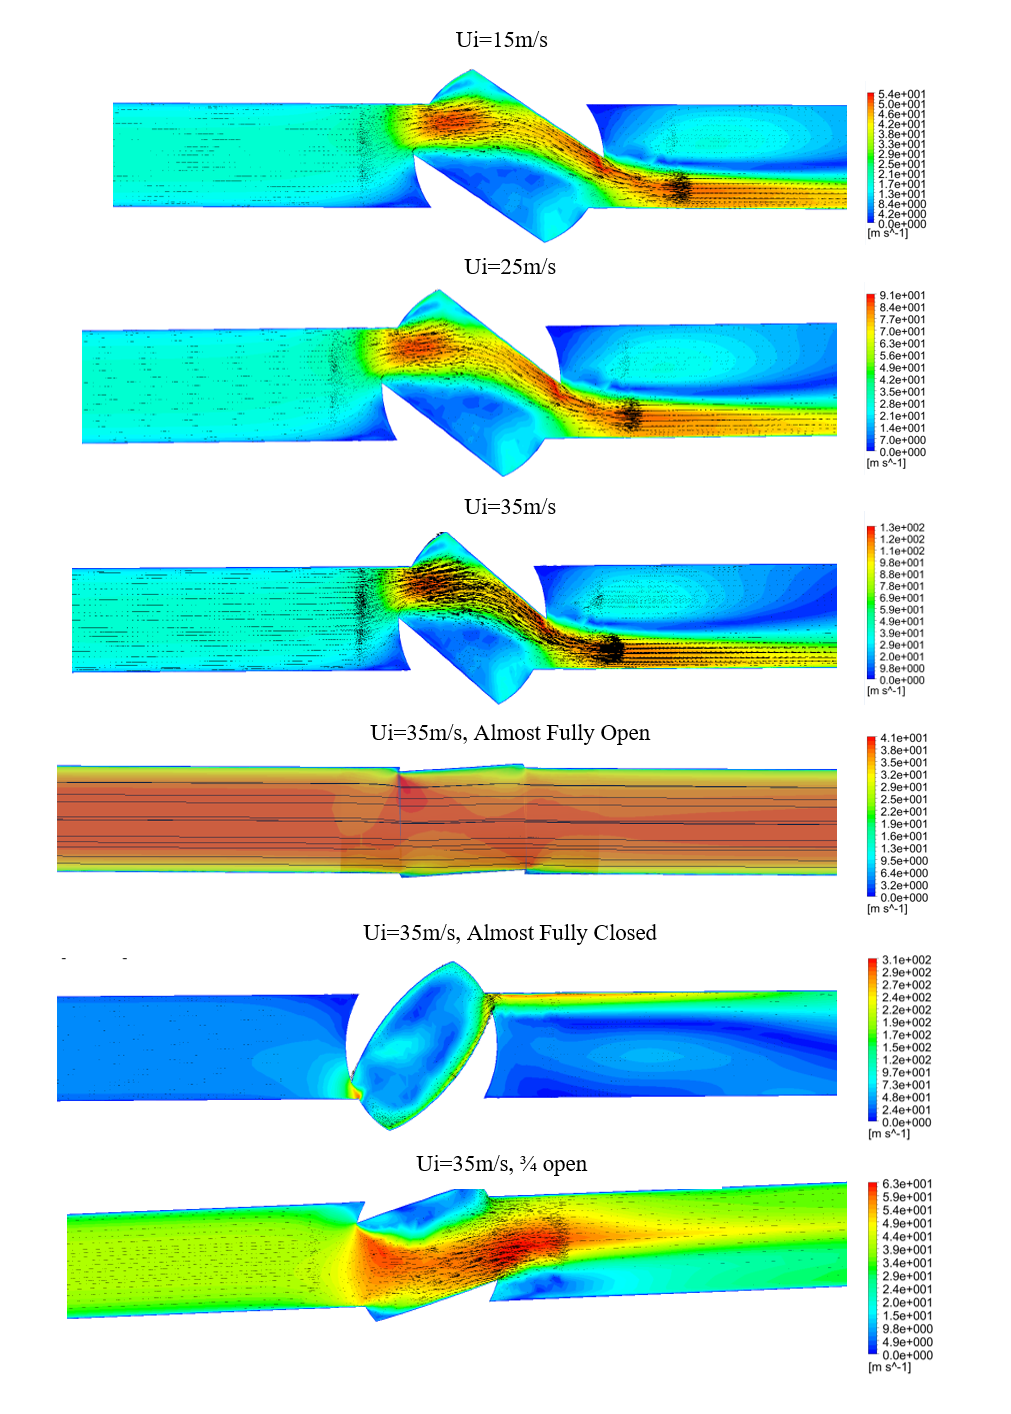
\includegraphics[width=0.7\linewidth]{Photos/Velocity}
	\caption{Velocity Contours for Different Configurations}
	\label{fig:velocity}
\end{figure}

\begin{figure}
	\centering
	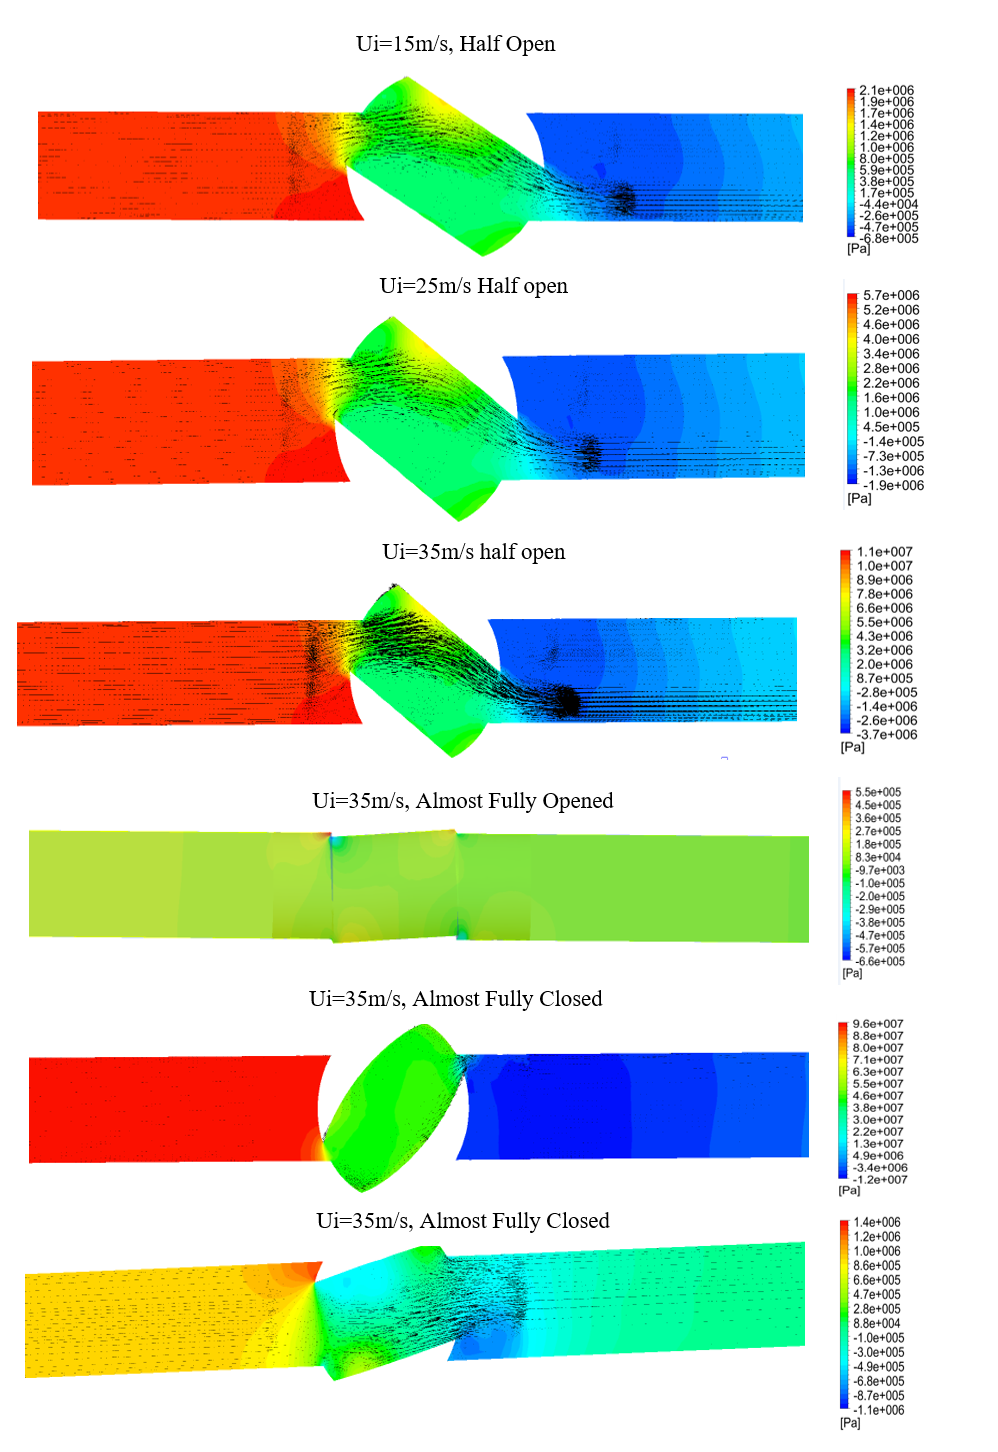
\includegraphics[width=0.7\linewidth]{Photos/Pressure}
	\caption{Static Pressure Contours for Different Inlets}
	\label{fig:pressure}
\end{figure}

\section{Discussion}
The various erosion patterns observed clearly indicate that this valve was continually operated in a partially opened condition between 30 to 50 rotational degrees from fully closed. In typical ball valve applications, failure occurs when the valve fails to seal and some amount of fluid is allowed to bypass the closed valve. In this application, the ball and seals were so severely damaged that they likely failed to seal for the majority of the valve's operational life. Thus, it is likely that this valve was being used as a throttling valve to control flow in an E/CRC experimental flow loop. It is assumed that the valve operated in this environment until the small pinhole formed in the valve body, at which point a leak would have been noticed and the valve replaced. Ball valves are generally not designed for continued throttling, and most, if not all, of the damage observed can be attributed to this misuse.

\subsection{General Erosion}
In typical ball valve applications, erosion from water flow and particle impact is minimal. When fully opened, the fluid flows through the valve unimpeded, and erosion rates are similar to those of straight pipe. When fully closed, no fluid flows so erosion is not present. However, severe erosion occurs when a ball valve is operated in the partially opened state. As water enters the partially opened valve, a concentrated area of high velocity flow forms at the valve wall. The valve interior is composed of a relatively soft brass alloy, and material is eroded rapidly from both the ball interior (Figure \ref{fig:internalballerossion}) and valve body (Figure \ref{fig:bodysides}). Eventually, enough material has been removed for water to flow around the backside of the ball. This flow continues until it reaches the sealed downstream surface and is diverted up or down around the ball. The resulting grooves are clearly seen in the valve body undercutting the seal (Figure \ref{fig:bodysides}) and on the ball (Figure \ref{fig:ball}(c)). At the outlet, severe erosion is observed as water impacts the right edge of the outlet seal (Figure \ref{fig:outletseal})) and exits the valve (Figure \ref{fig:bodyoutlet}). 

In this valve, damage produced by general erosion appears smooth and shiny. This occurs because the high erosion rate continually removes surface corrosion, exposing uncorroded brass. 

\subsection{Abrasion}
The valve shows signs of extensive damage from abrasive wear. The debris on both the inlet and outlet seals contains silicon particles that suggest the presence of sand in the fluid. In addition to increasing the rate of general fluid erosion, sand granules of various sizes were embedded in the seal surface as water entered the valve (Figure \ref{fig:inletseal}, water inflow region). As the valve was opened and closed, the sand scratched the ball surface, as evidenced by the parallel gouge marks on the ball sealing faces (Figure \ref{fig:ball}). It is worth noting that without heat treatment, nickel coatings are less hard than silicon sand. Unlike the channels formed by pure erosion, these channels tended to be darker and rougher in appearance due to corrosion that was not rapidly removed by the fluid. The depth of the scratch marks indicate that the valve was adjusted frequently, which further supports the throttling assumptions above.

While not completely eliminated, the abrasive damage due to hard particles is drastically reduced when ball valves are operated as shutoff valves. When a ball valve is fully opened or closed, the seals are not exposed to the particles within the flow. During throttling, the seal is continually exposed, which increases the number of particles that can become embedded in the seal surface.

\subsection{Corrosion}
SEM EDS indicated trace amounts of sodium and chlorine on both the ball and seal surfaces, suggesting the presence of salt in the fluid. According to a study conducted by Zhang \cite{Zhang2009}, the presence of chlorine ions expedites a corrosion process known as dezincification. During this process, zinc reacts to form oxides that are mechanically removed from the surface leaving behind a porous, rough copper surface. This is seen in the dark portions of the ball (Figure \ref{fig:ball}(a)(d)) and valve body (Figure \ref{fig:inlet}(b)). Dezincification occurs in brass alloys with zinc concentrations above \verb|15%|. Per the valve manufacturer data sheet, the brass alloy in this valve is C28500, which contains approximately \verb|60%| copper and \verb|40%| Zinc with  trace amounts of iron and lead. This is consistent with the values obtained from the SEM EDS of the uncorroded portion of the ball in Figure \ref{fig:BallSEM}. While this composition is ideal for forging, the high zinc content makes it extremely susceptible to dezincification. SEM EDS indicated little to no zinc in corroded areas, which suggests that dezincification has occurred. This type of corrosion is typically most severe in areas of low velocity flow, which is consistent with shiny surfaces in regions of high flow and erosion.

\subsection{Cavitation}
During throttling, static pressure in the valve may fall below the water vapor pressure causing rapid vaporization. This results in cavitation and bubble formation. When the fluid pressure increases above the vapor pressure, the bubbles collapse and emit tiny shock waves into the fluid. Damage caused by these shock waves is known as cavitation erosion. This type of erosion is characterized by random pock marks seen in Figures \ref{fig:ball}(a)(d), \ref{fig:bodyside2}. Cavitation erosion is also the primary cause of damage to the inlet seal mixed contact region (Figure \ref{fig:inletseal}).

\section{Conclusions}
The 1/4" ball valve from the University of Tulsa's North Campus showed signs of extreme internal damage. The first sign of failure is assumed to be leakage from the valve body. The valve was operated in a partially open state to throttle flow in an experimental E/CRC loop. Throttling increased fluid velocity at the wall and caused excessive erosion of the casing and ball. Operating the valve in a partially opened state allowed sand particles to become embedded in the sealing surfaces, causing abrasive damage to the ball during valve adjustment. Chlorine ions weakened the brass components through a corrosive process known as dezincification. Throttling created regions of extremely low pressure causing fluid cavitation. These failure modes can be mitigated by operating the valve in the fully open or fully closed positions. 

\section{Recommendations}

\subsection{Alternative Valve Selection}
Ball valves are an economical choice for shutoff applications. However, as this study has shown, ball valve design makes them a poor choice for throttling applications. A suitable alternative commonly used in industry is a globe-type valve (Figure \ref{fig:GlobeValve}). 
\begin{figure}[h]
	\centering
	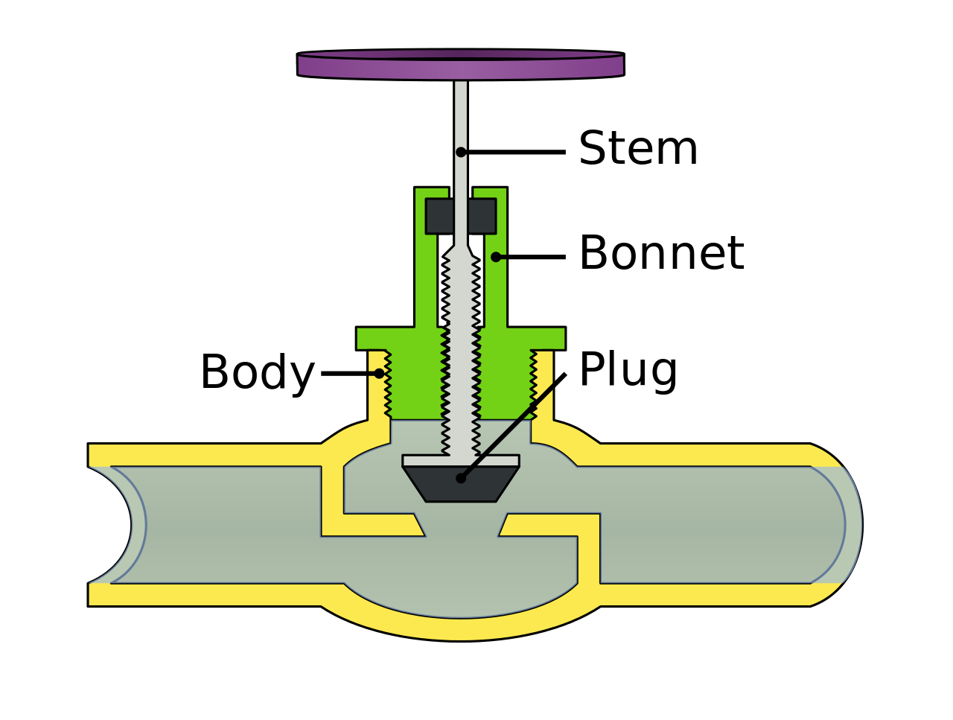
\includegraphics[width=0.7\linewidth]{Photos/GlobeValve}
	\caption{Globe Valve Design (Oil and Gas Club \cite{OilandGasClub})}
	\label{fig:GlobeValve}
\end{figure}

\subsection{Economic Considerations}
Ball valves are typically less expensive than globe valves, but the replacement rate is expected to be higher.  For 1/4" valves, the difference in price is inconsequential compared to the cost of other system components. However, since the ball valve continued to function beyond its "normal" failure point (failing to seal), a comparison test may be warranted for larger valves.

\subsection{Safety Considerations}
Ball valves are inappropriate for throttling hazardous fluids, since the first noticeable sign of failure is fluid leakage. Additionally, ball valves whose shutoff function is relied on for safety purposes should not be used to throttle fluid. In certain applications where contamination might pose a risk to consumers, dezincification should be controlled by selection of alternative alloys (see valve improvement). If ball valves are being used to throttle hazardous fluids, they should be routinely inspected and replaced.

\subsection{Valve Design}
The following design improvements have been identified to counteract the various failure modes observed.
\begin{enumerate}
	\item Heat treat the nickel plating to a value harder than that of sand.
	\item Use a brass with less than \verb|15%| zinc or add alloying elements to prevent dezincification. 
	\item Replace valves that have failed to perform any of their designed functions.
\end{enumerate}

%\pagebreak
\bibliographystyle{plain}
\bibliography{Bibli}

\end{document}